\documentclass[10pt]{beamer}
\usetheme[
%%% options passed to the outer theme
%    hidetitle,           % hide the (short) title in the sidebar
%    hideauthor,          % hide the (short) author in the sidebar
%    hideinstitute,       % hide the (short) institute in the bottom of the sidebar
%    shownavsym,          % show the navigation symbols
%    width=2cm,           % width of the sidebar (default is 2 cm)
%    hideothersubsections,% hide all subsections but the subsections in the current section
%    hideallsubsections,  % hide all subsections
%    left                % right of left position of sidebar (default is right)
  ]{Aalborg}
  
% If you want to change the colors of the various elements in the theme, edit and uncomment the following lines
% Change the bar and sidebar colors:
%\setbeamercolor{Aalborg}{fg=red!20,bg=red}
%\setbeamercolor{sidebar}{bg=red!20}
% Change the color of the structural elements:
%\setbeamercolor{structure}{fg=red}
% Change the frame title text color:
%\setbeamercolor{frametitle}{fg=blue}
% Change the normal text color background:
%\setbeamercolor{normal text}{bg=gray!10}
% ... and you can of course change a lot more - see the beamer user manual.

\usepackage[utf8]{inputenc}
%\usepackage[english]{babel}
\usepackage[spanish]{babel}
\usepackage[T1]{fontenc}
\usepackage[demo]{graphicx}   
% Or whatever. Note that the encoding and the font should match. If T1
% does not look nice, try deleting the line with the fontenc.

\usepackage[table,xcdraw]{xcolor}
\usepackage{helvet}
\usepackage{tikz}
\usetikzlibrary{shapes,arrows,positioning}

%\usepackage{minted}
\usepackage{animate}
\usepackage{media9}


\usepackage{listings}
\usepackage{color}
\definecolor{codegreen}{rgb}{0,0.6,0}
\definecolor{codegray}{rgb}{0.5,0.5,0.5}
\definecolor{codepurple}{rgb}{0.58,0,0.82}
\definecolor{backcolour}{rgb}{0.95,0.95,0.92}
 
\lstdefinestyle{mystyle}{
    backgroundcolor=\color{backcolour},   
    commentstyle=\color{codegreen},
    keywordstyle=\color{magenta},
    numberstyle=\tiny\color{codegray},
    stringstyle=\color{codepurple},
    basicstyle=\footnotesize,
    breakatwhitespace=false,         
    breaklines=true,                 
    captionpos=b,                    
    keepspaces=true,                 
    numbers=left,                    
    numbersep=5pt,                  
    showspaces=false,                
    showstringspaces=false,
    showtabs=false,                  
    tabsize=2
}
 
\lstset{style=mystyle}


% colored hyperlinks
\newcommand{\chref}[2]{%
  \href{#1}{{\usebeamercolor[bg]{Aalborg}#2}}%
}

\title[Análisis y Diseño de Circuitos Eléctricos]% optional, use only with long paper titles
{Análisis y Diseño de Circuitos Eléctricos}

\subtitle{Cantidades eléctricas fundamentales, notación científica y unidades eléctricas estándar}  % could also be a conference name

\date{\today}

\author[Víctor Medrano Zarazúa] % optional, use only with lots of authors
{
  Víctor Medrano Zarazúa\\
  \href{mailto:victor_medrano@my.uvm.edu.mx}{{\tt victor\_medrano@my.uvm.edu.mx}}
}
% - Give the names in the same order as they appear in the paper.
% - Use the \inst{?} command only if the authors have different
%   affiliation. See the beamer manual for an example

\institute[
%  {\includegraphics[scale=0.2]{aau_segl}}\\ %insert a company, department or university logo
  %Dept.\ of Electronic Systems\\
  Universidad del Valle de México\\
  Campus Monterrey
] % optional - is placed in the bottom of the sidebar on every slide
{% is placed on the bottom of the title page
  %Department of Electronic Systems\\
  Universidad del Valle de México\\
  Campus Monterrey
  %Universidad Autónoma de Nuevo León\\
  %Facultad de Ingeniería Mecánica y Eléctrica
  
  %there must be an empty line above this line - otherwise some unwanted space is added between the university and the country (I do not know why;( )
}

% specify the logo in the top right/left of the slide
\pgfdeclareimage[height=1cm]{mainlogo}{AAUgraphics/UVM} % placed in the upper left/right corner
\logo{\pgfuseimage{mainlogo}}

% specify a logo on the titlepage (you can specify additional logos an include them in 
% institute command below
\pgfdeclareimage[height=1.5cm]{titlepagelogo}{AAUgraphics/UVM} % placed on the title page
%\pgfdeclareimage[height=1.5cm]{titlepagelogo2}{AAUgraphics/aau_logo_new} % placed on the title page
\titlegraphic{% is placed on the bottom of the title page
  \pgfuseimage{titlepagelogo}
%  \hspace{1cm}\pgfuseimage{titlepagelogo2}
}

%\definecolor{UniBlue}{RGB}{255,255,255}

\tikzset{
block/.style={
  draw, 
  fill=blue!20, 
  rectangle, 
  minimum height=3em, 
  minimum width=6em
  },
 gain/.style={
    draw,
    fill=blue!20, 
    isosceles triangle,
    minimum height = 3em,
    isosceles triangle apex angle=60
    },
sum/.style={
  draw, 
  fill=blue!20, 
  circle, 
  },
input/.style={coordinate},
output/.style={coordinate},
pinstyle/.style={
  pin edge={to-,thin,black}
  }
}  

\begin{document}
% the titlepage


%\setbeamercolor{title}{fg=UniBlue}
%\setbeamercolor{normal text}{fg=UniBlue}
%\setbeamercolor{Aalborg}{fg=black,bg=black}


{\aauwavesbg
\begin{frame}[plain,noframenumbering] % the plain option removes the sidebar and header from the title page
  \titlepage
\end{frame}}
%%%%%%%%%%%%%%%%

% TOC
\begin{frame}{Contenido}{}
\tableofcontents
\end{frame}
%%%%%%%%%%%%%%%%
\section{Repaso}
\begin{frame}{Repaso}{}
\begin{block}{Recapítulemos...}
\begin{itemize}
\item ¿Qué es la carga eléctrica y cuál es su unidad de medida?
\item ¿Cuál es la diferencia entre conductor, aislante y seminconductor?
\item Menciona ejemplos de conductores, aislantes y semiconductores.
\item ¿Qué es la corriente eléctrica y cuál es su unidad de medida?
\end{itemize}
\end{block}

\end{frame}

\begin{frame}{Repaso}{}
\begin{block}{Recapítulemos...}
\begin{itemize}
\item ¿Cuál es la diferencia entre corriente eléctrica real y corriente eléctrica convencional?
\item ¿Cuál es la diferencia entre transportar corriente eléctrica en un metal y transportar corriente eléctrica en un solución de agua y sal?
\item ¿Qué es el voltaje y cuál es su unidad de medida?
\item ¿Qué representa una ecuación diferencial en el mundo real?
\end{itemize}
\end{block}

\end{frame}


%\begin{frame}{Introducción}{}
%\begin{block}{Tenemos tecnología...}
%\begin{itemize}
%Hoy vivimos en un mundo predominantemente eléctrico. Las dos áreas primarias de la electrotecnología que permean esencialmente todos los aspectos de nuestras vidas son la potencia y la información.
%\end{itemize}
%\end{block}

%\begin{figure}[h!]
%\centering
%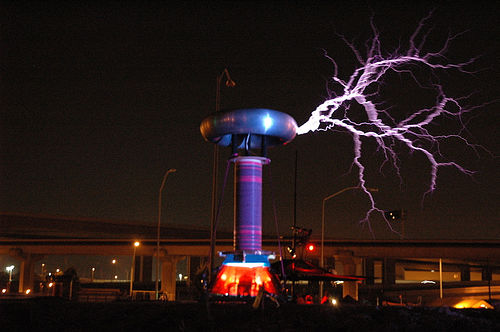
\includegraphics [scale=0.32]{teslacoil}
%\caption{Bobina Tesla}
%\label{fig:tesla}
%\end{figure}
%\end{frame}

\section{Introducción}
%\section{Carga eléctrica}
\begin{frame}{Introducción}{}

\begin{block}{Amamos los números}
\begin{itemize}
    \item Los ingenieros lidiamos día a día con los números. Estos números pueden ser muy pequeños o muy grandes.
    \item Los ingenieros somos un poco perezosos al momento de escribir números, así que los abreviamos.
    \item En la ingeniería, los números se escriben en notación de ingeniería, que es similar a la notación científica.
\end{itemize}
\end{block}

\end{frame}

\section{Notación científica}

\begin{frame}{Notación científica}{O como escribir números pequeñitos y grandototes}
\begin{block}{Número de Avogadro}
\begin{itemize}
    \item Un número muy utilizado en Química y que describe la cantidad de átomos o moléculas en una cantidad de sustancia de un mol es el número de Avogadro: 602200000000000000000000.
    \item Es difícil decir el nombre de este número al momento de leerlo.
    \item Y no hablemos de escribirlo.
\end{itemize}
\end{block}
\end{frame}

\begin{frame}{Notación científica}{O como escribir números pequeñitos y grandototes}

\begin{block}{Potencias de 10}
Antes de abreviar el número de Avogadro, veamos el resultado de elevar 10 a distintas potencias.
\end{block}
\medskip
\begin{columns}[c]
\column{1.8in}
\framebox{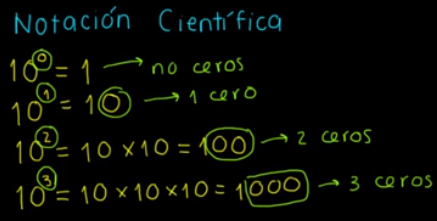
\includegraphics[width=1.8in]{notcien}}
\column{1.8in}
\framebox{\href{https://www.youtube.com/watch?v=97CWXZa66C4}{
\includegraphics[width=1.8in]{googol}}}
\end{columns}
\end{frame}

\begin{frame}{Notación científica}{O como escribir números pequeñitos y grandototes}

\begin{block}{Potencias de 10}
Un número está escrito en notación científica cuando hay un número mayor que o igual a 1 pero menor que 10 multiplicado por una potencia de 10.
Abreviamos el número de Avogadro usando potencias de 10. Ver \href{https://es.khanacademy.org/math/pre-algebra/pre-algebra-exponents-radicals/pre-algebra-scientific-notation/e/scientific_notation}{\textcolor{blue}{ejercicio}}.
\end{block}
\medskip
\begin{figure}[h!]
\centering
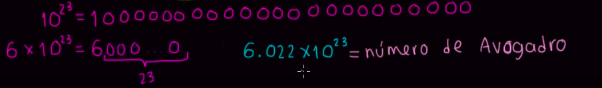
\includegraphics [scale=0.39]{avogadro}
\label{fig:first}
\end{figure}
\end{frame}

\begin{frame}{Notación científica}{Algunos números importantes}
\begin{block}{Datos interesantes}
\begin{itemize}
    \item La velocidad de la luz es 299792458299792458299792458 metros por segundo.
    \item La carga del electrón es un número muy pequeño y difícil de manejar: 0.00000000000000000016021766208 coulombs.
\end{itemize}
\end{block}

\end{frame}

\section{Notación de ingeniería}

\begin{frame}{Notación de ingeniería}{Modificando la notación científica}
\begin{block}{Nos gustan los exponentes en múltiplos de tres}
A la luz le lleva 0.0000333564095 segundos recorrer 10 kilómetros en el vacío. Vamos a expresar este pequeño número en notación de ingeniería:

\begin{itemize}
    \item Encuentra el punto decimal.
    \item Salta sobre tres cifras a la vez, yendo a la derecha, hasta que saltes sobre uno, dos o tres dígitos diferentes de cero. En este caso, haz dos saltos a la derecha, hasta saltar sobre 33.
    \item Escribe 33.
    \item Añade un punto decimal: 33.
    \item Escribe los dígitos restantes: 33.3564095.
    \item Debido a que saltamos a la derecha, escribe 10 elevado al negativo del número de saltos multiplicado por tres: $-2 \times 3 = -6$.
\end{itemize}
\end{block}
\end{frame}

\begin{frame}{Notación de ingeniería}{Modificando la notación científica}
\begin{block}{Prefijos}
Muchos números tienen nombres derivados del griego o del latín. Los ingenieros y científicos utilizan prefijos para los números de acuerdo con lo establecido en el Système International d'Unités (SI).
\end{block}

\begin{figure}[h!]
\centering
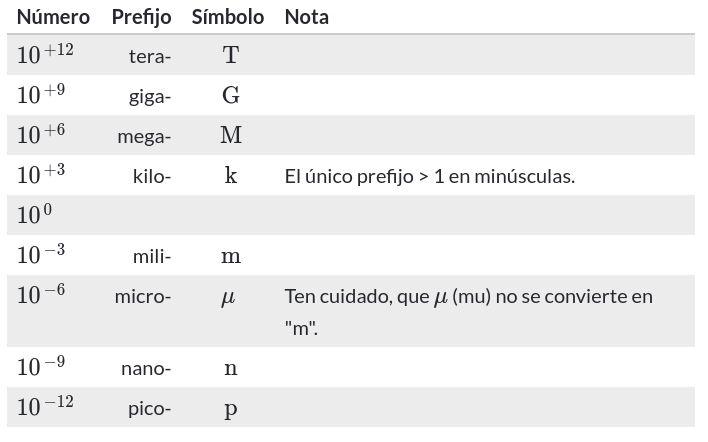
\includegraphics [scale=0.32]{prefix}
\label{fig:first}
\end{figure}

\end{frame}

\section{Escribiendo unidades}

\begin{frame}{Gramática de las unidades}{}
\begin{block}{Nombres y símbolos}
\begin{itemize}
    \item Los nombres de todas las unidades comienzan con una letra minúscula, incluso si la unidad se nombra en honor a una persona.
    \item Los símbolos para las unidades son mayúsculas si la unidad lleva el nombre de una persona; de lo contrario son minúsculas.
\end{itemize}
\end{block}

\begin{figure}[h!]
\centering
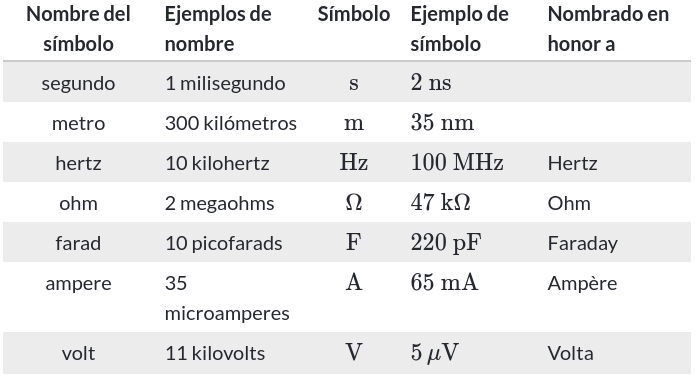
\includegraphics [scale=0.28]{gram}
\label{fig:first}
\end{figure}

\end{frame}

%%%%%%%%%%%%%%%%%%%%%%%%%%%%5
\section{Información de contacto}
% contact information
\begin{frame}{Feedback}{Información de contacto}
En caso de comentarios, sugerencias, preguntas o errores en las diapositivas no dudes en contactarme.
  \begin{center}
    \insertauthor\\
    \chref{https://mixlaab.github.io}{https://mixlaab.github.io}\\
    WA: 8119022700\\
    %9220 Aalborg Ø
  \end{center}
\end{frame}
%%%%%%%%%%%%%%%%

{\aauwavesbg%
\begin{frame}[plain,noframenumbering]%
  \finalpage{Fin}
\end{frame}}
%%%%%%%%%%%%%%%%

\end{document}
